\begin{figure}[H]
	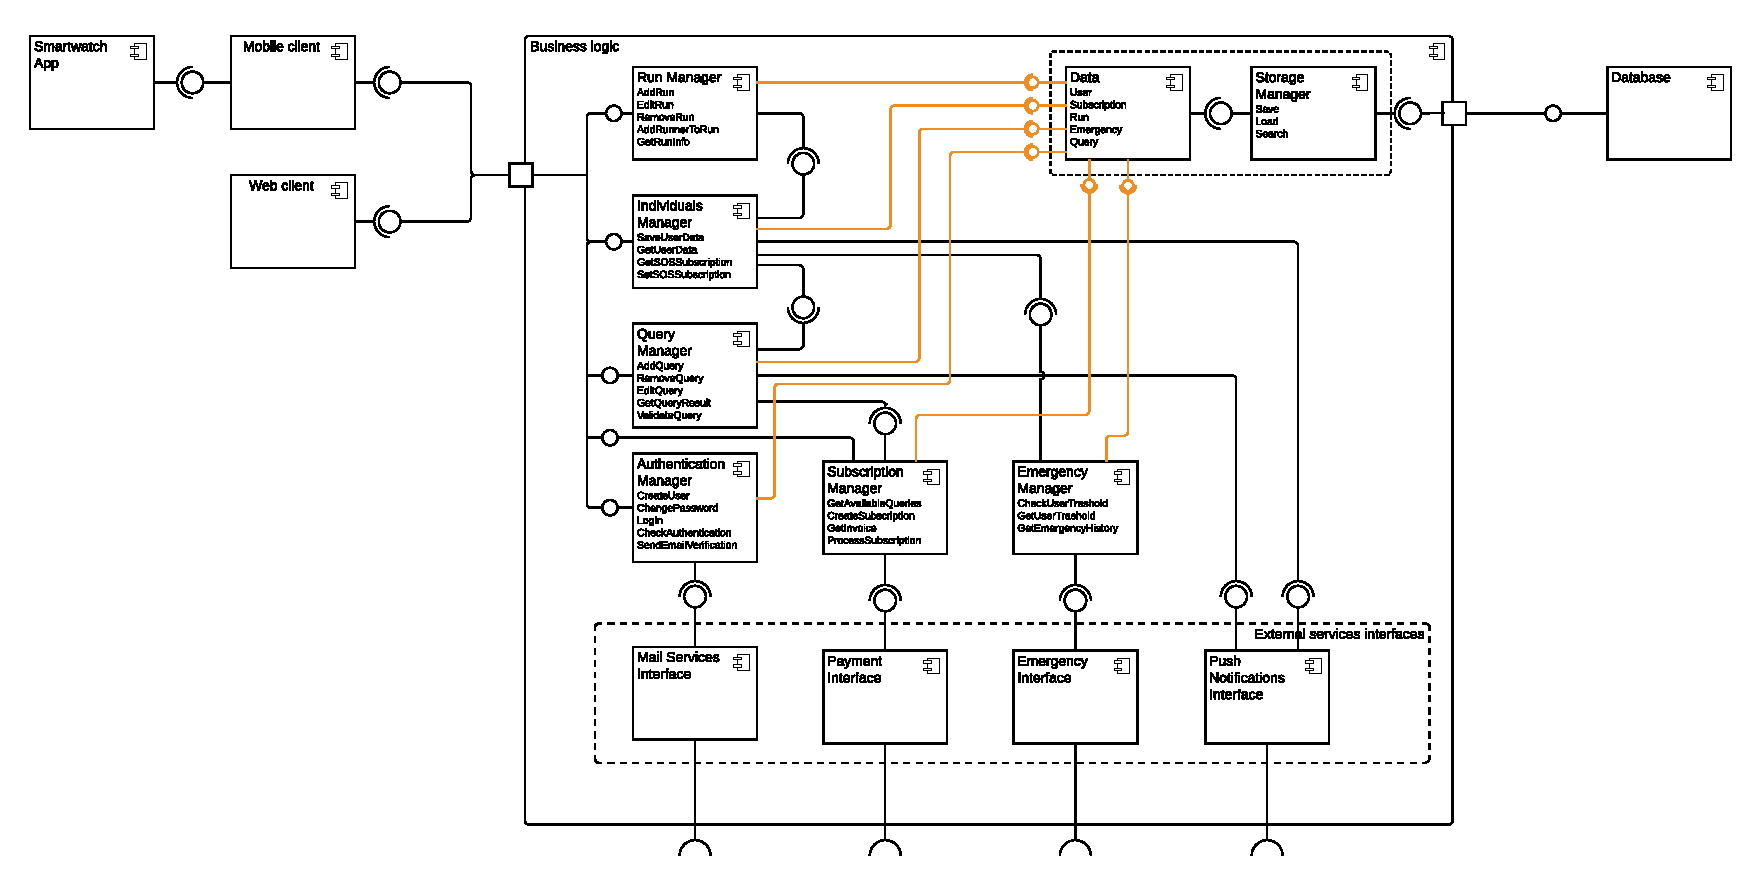
\includegraphics[width=\textwidth,height=\textheight,keepaspectratio]{assets/ComponentDiagram.pdf}
	\caption{Component Diagram}
	\label{fig:CD}
\end{figure}


\noindent The picture shows the components of the application divided in Client, Business Logic and Data tier.

\noindent Below are described more in detail all the components and interfaces that the system uses to offer its functionalities.

\paragraph{Smartwatch device} \mbox{} \newline
The Smartwatch device is directly connected to the mobile app of the user and does not interact with the business logic.
Data coming from the sensors of the smartwatch are sent to the mobile app via bluetooth.

\paragraph{Mobile client and Web client} \mbox{} \newline
The clients of the system.
\begin{itemize}
    \item The Mobile client is used by individuals that want to exploit the services of Data4Help.
    \item The Webclient is used by Companies that want to exploit the query services of Data4Help.
\end{itemize}


\paragraph{Individuals Manager} \mbox{} \newline
The Individuals manager has to 
\begin{itemize}
    \item notify the system when there are new data available and store them into it;
    \item manage user requests for historical data, accessing Data4help database;
    \item ask the user if he agrees to be monitored by a company that has requested an individual query, sending him a push notification;
    \item communicate data to Emergency manager (only if user is subscribed to AutomatedSOS);
\end{itemize}


\paragraph{Authentication Manager} \mbox{} \newline
The component that manages users log-in and registration and is in charge of:
\begin{itemize}
    \item allowing user login;
    \item changing user authentication information;
    \item adding new user to database;
    \item communicating with Email interface in order to send verifications request to the user
\end{itemize}

\paragraph{Query Manager} \mbox{} \newline
The core component of the Business unit. It is in charge of:
\begin{itemize}
    \item \textbf{Get query results};
    \item \textbf{Validating queries}: verify if there is a sufficient number of users involved in the scope of the query (in case of a query on group of individuals), and if a company is allowed to do a query according to its payment subscription;
    \item \textbf{Adding queries} to a company account;
    \item \textbf{Deleting queries} from a company account that wish to unsubscribe
    \item \textbf{Updating queries}, when a company has subscribed to a query and wants to edit its query; interacts with the Push Notification interface to send the "New data" notification.
\end{itemize}

\paragraph{Subscription Manager} \mbox{} \newline
The component is in charge of managing the subscription of companies to a payment plan offered by Data4Help.
It has to:
\begin{itemize}
    \item \textbf{Subscribe}: let companies subscribe to new payment plans;
    \item \textbf{Store} in the database subscriptions of every company;
    \item \textbf{Let companies see} their subscription detail;
    \item \textbf{Interact} with the payment service to let company pay for subscriptions.
\end{itemize}



\paragraph{Emergency Manager} 
\mbox{} \newline
The component is in charge of 
\begin{itemize}
    \item \textbf{Evaluating} user health parameters;
    \item \textbf{Store} in the database threshold parameters for users subscribed to AutomatedSOS;
    \item \textbf{Checking} when a parameter of a user goes below the threshold. If so, the component is in charge to communicate with ambulance API throughout the Emergency interface.
\end{itemize}


\paragraph{Run Manager} \mbox{} \newline
The component is in charge of:
\begin{itemize}
    \item \textbf{Creating races}: allows run organizers to create new races;
    \item \textbf{Listing run}: provides a list of runs be available to users;
    \item \textbf{Adding} new runners to a race;
    \item \textbf{Managing}: let run organizers manage a race's information.
\end{itemize}


\paragraph{External services interface} \mbox{} \newline
The system has 3 interfaces components that are in charge of communicating with the external services API.
The interfaces are:
\begin{itemize}
    \item Push Notification Interface: communicates with a push notification server API in order to send notifications to mobile client;
    \item Emergency Services Interface: communicates with Ambulance API provided by Hospitals in order to send an ambulance if the user health parameters go below thresholds;
    \item Mail Services Interface: communicates with email server to send email.
    \item Payment Interface: communicates an external payment service in order to create payment requests and validate them.
\end{itemize}

The diagram below describes in details the components and the entities of the application server.


\begin{figure}[H]
	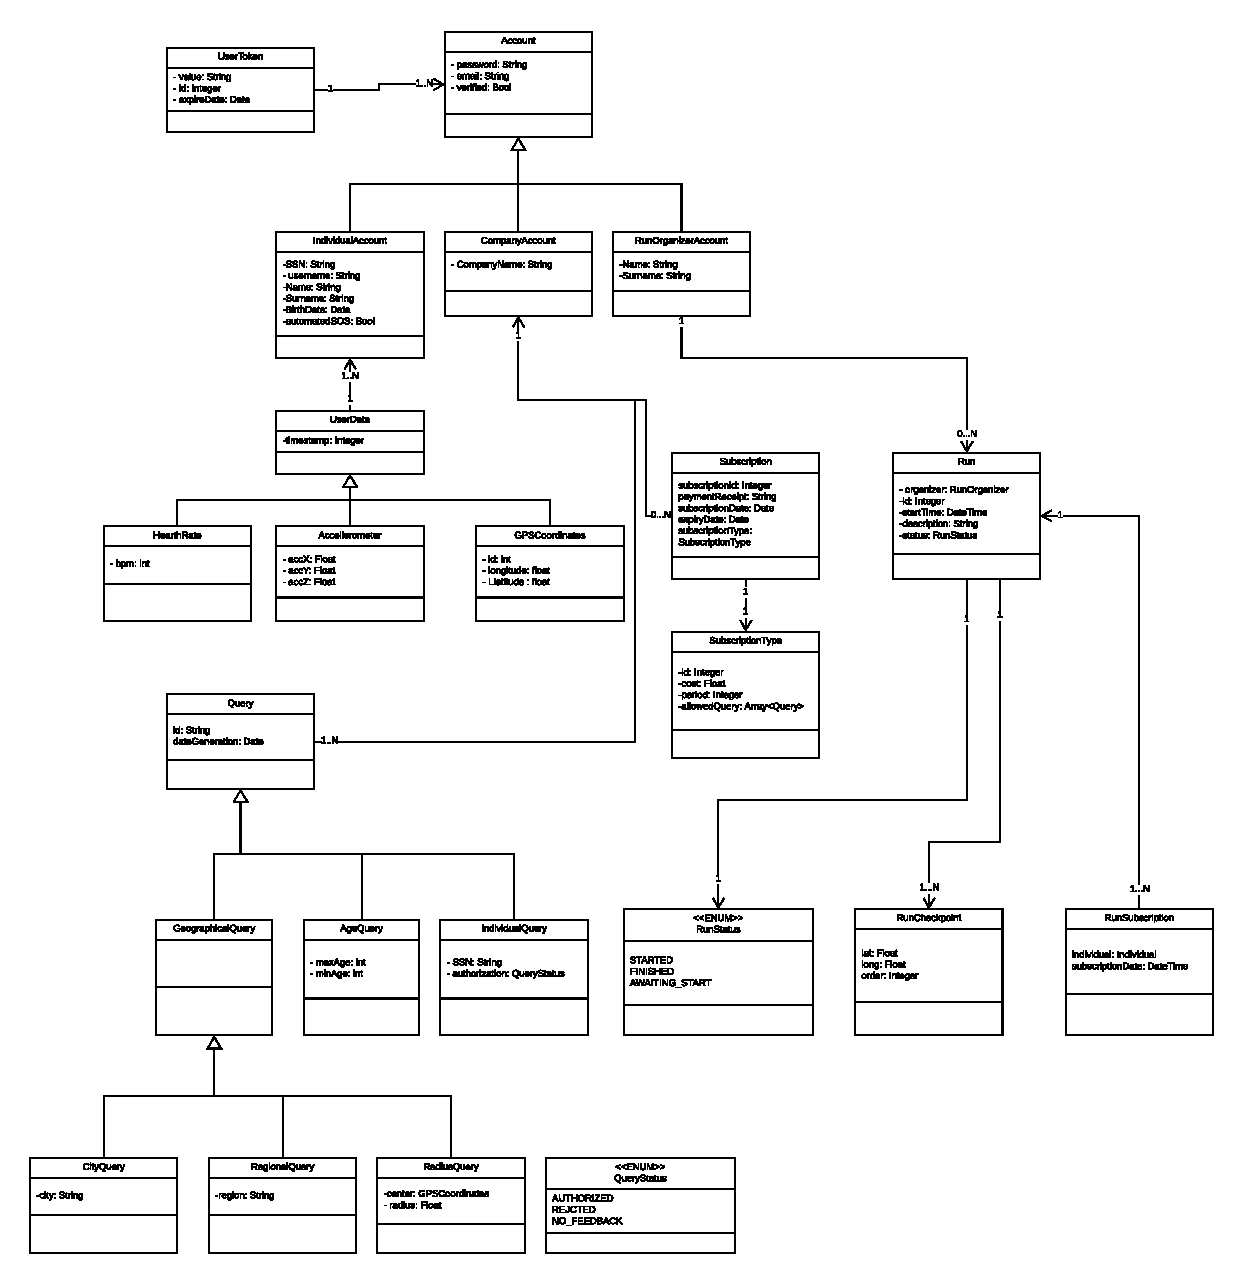
\includegraphics[width=\textwidth,height=\textheight,keepaspectratio]{assets/UML_Entities.pdf}
	\caption{Entities diagram}
	\label{fig:UMLEntityDiagrams}
\end{figure}
